\documentclass{article}
\usepackage[utf8]{inputenc}
\usepackage[T1]{fontenc}
\usepackage{graphicx}
\usepackage{hyperref}
\usepackage{geometry}
\geometry{margin=1in}

\title{SILLESIAN EARTH}
\date{Encyclopaedia Britannica (1771)}

\begin{document}
\maketitle

\section*{Historical source}
\textbf{Entry ID:} \texttt{entry-sillesian-earth-2001} \\
\textbf{Volume ID:} 192200899 \\
\textbf{Character Count:} 495

\subsection*{Extracted Text}
SILLESIAN EARTH, in the \_Materia Medice\_, a fine affungent bole. It is very heavy, of a firm compel tantras, and in colors of the brownie yellow. It breaks early between the fingers, and does not flash the hands; is naturally a smooth before, is readily available in water, and multis freely into a butterflies, lightable in the mouth. It leaves no grittiness between the teeth, and does not ferment with acids. It is found in the perpendicular letters of rocks across the gold mines in Hungary.



\section*{Source record}
\begin{itemize}
\item \textbf{Dataset:} \texttt{NationalLibraryOfScotland/encyclopaedia\_britannica\_illustrated}
\item \textbf{Dataset Revision:} \texttt{309f765b1ecc83e0a7f7762e44b4a927a7555443}
\item \textbf{Page ID:} \texttt{britannica:309f765b1ecc83e0a7f7762e44b4a927a7555443:train:2001} \\
  \textbf{Filename:} \texttt{page-2001-93040a5ab362.jpg} \\
  \textbf{Row Index:} 2001 \\
  \textbf{SHA256:} \texttt{93040a5ab3625efc...}
\end{itemize}

\begin{figure}[h]
\centering
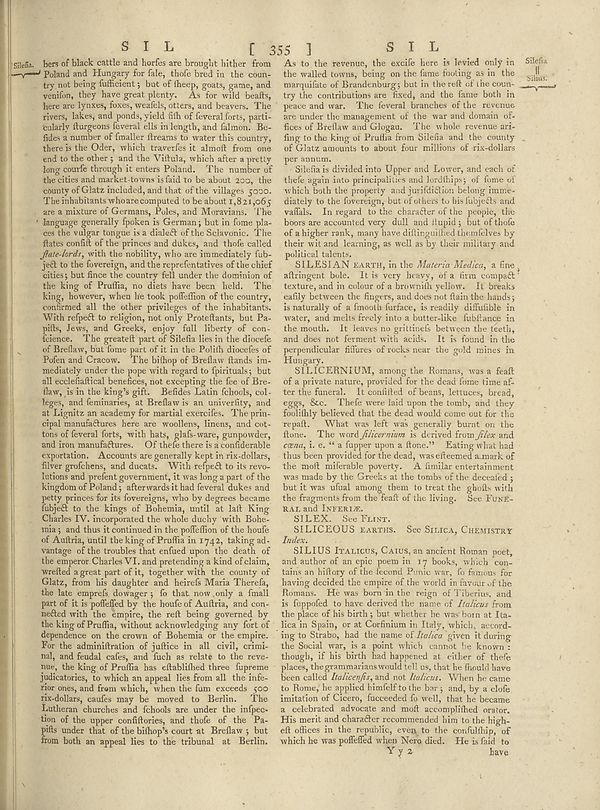
\includegraphics[width=0.85\textwidth]{../scans/page-2001-93040a5ab362.jpg}
\caption*{Source scan: \texttt{page-2001-93040a5ab362.jpg}}
\end{figure}

\end{document}
